%\documentclass[a4paper,12pt]{article}
%\usepackage{graphicx}
%\usepackage{amsmath}
%\usepackage{amsfonts}
%\usepackage{geometry}
%\usepackage{fancyhdr}
%\usepackage{color}
%\usepackage{tikz}
%\usetikzlibrary{shapes.geometric, arrows}
%
%\tikzstyle{startstop} = [rectangle, rounded corners, minimum width=3cm, minimum height=1cm, text centered, draw=black, fill=red!30]
%\tikzstyle{process} = [rectangle, minimum width=3cm, minimum height=1cm, text centered, draw=black, fill=blue!30]
%\tikzstyle{arrow} = [thick,->]
%
%
%\usepackage{hyperref}
%\usepackage[natbib=true,style=authoryear,backend=biber,useprefix=true]{biblatex}
%\geometry{margin=1in}
%\pagestyle{fancy}
%\fancyhf{}
%\rhead{Project Report}
%\lhead{ESP32-CAM Face Recognition}
%\cfoot{\thepage}
%\addbibresource{Literature.bib}
%
%
%
%\begin{document}
%\begin{titlepage}
%	
%	\begin{flushleft} 
%		
\includegraphics[width=7cm]{Applications/ESP32FaceRecognition/logo.jpg}
%	\end{flushleft} 
% \vspace{1cm}
%	
%	\begin{flushright}
%
%		\LARGE \textsl{Homework}\\
%		\rule{0.6\textwidth}{0.4pt} ~\\
%		\textsf{\LARGE\textbf{Results: Face Recognition using ESP32-CAM SPECIAL}}\\ [0.5cm]
%	\end{flushright}
%	
%	\large
%	\begin{tabbing}
%		xxxxxxxxxxxxxxxx \= \kill
%		Student : \> Danish Husain Saiyed \\ 
%		Matrikel-No.: \> 7026369 \\ [0.75cm]
%		Study Program: \> Industrial Informatics \\  [0.75cm]
%  
%            Professor: \> Prof. Dr. Elmar Wings \\
%                        [0.75cm]
%	        Date: \> \today \\
%    \end{tabbing}
%	\vspace{0.9cm}
%	\small
%	\begin{center}
%		Hochschule Emden/Leer $\cdot$ 
%		%Fachbereich Technik $\cdot$ 
%		Industrial Informatics \\
%		Constantiaplatz 4 $\cdot$ 
%		26723 Emden $\cdot$ 
%		\url{http://www.hs-emden-leer.de}
%	\end{center}
%	
%\end{titlepage}
%
%\tableofcontents
%\newpage

\section{Introduction}
In the rapidly evolving world of embedded systems and artificial intelligence, the convergence of edge computing with real-time decision-making has become a cornerstone for many applications. Among them, face recognition systems stand out for their usefulness in automation, security, and smart environments. This report presents a comprehensive overview of a face recognition solution implemented using the ESP32-CAM SPECIAL module. The goal of this project was to develop a compact, low-cost, and efficient system that captures, processes, and recognizes human faces using embedded hardware without the need for high-performance computing infrastructure. 

The project journey covers multiple phases including domain research, understanding data processing workflows, setting up development environments, implementing real-time inference models, and deploying them on embedded hardware. Through the integration of Edge Impulse for model training and Arduino IDE for development, this report encapsulates a complete end-to-end lifecycle of a machine learning system at the edge.

The Espressif32 Camera Module (ESP32-CAM) is a  microcontroller with an Espressif32 (ESP32)-S development board along with an onboard
camera module and micro-Secure Digital (SD) card port. In addition, this board has
integrated Wireless Fidelity (WiFi) and Bluetooth Low Energy (BLE), which allows
it to transfer data wirelessly when required.\\

The ESP32-CAM is a development board that combines an ESP32-S chip, a
microcontroller with integrated WiFi and Bluetooth capability, with a camera module,
making it a compact solution for various Internet of Things (IoT) and Do It Yourself
(DIY) projects. This board integrates a 2 Megapixels (MP) camera and supports the
Arduino Integrated Development Environment (IDE), enabling easy programming and
interfacing with other devices.\\

The ESP32-CAM with its onboard capabilities and connectivity options, the ESP32-CAM
finds applications in surveillance systems, smart home automation, remote monitoring,
and other projects requiring both wireless communication and visual data acquisition. Its affordability, compact size, and extensive capabilities make it a popular
choice among hobbyists, developers, and enthusiasts exploring the realms of IoT and
embedded systems.\\

ESP32-CAM is readily available in different HW Distributors online with costs ranging
from around 10 Euros to 20 Euros, depending on other additional gadgets included,
such as Development Board, Serial Converter, and others required for larger scale
projects.\\

The small form factor, availability and economic feasibility of the ESP32 make it a
perfect solution for various IoT applications such as wireless monitoring, quick response
code identification, image tracking, image recognition, smart home devices, industrial
wireless control and other applications.\\

The ESP32-CAM is employed in this project due to its integrated camera and processing
capabilities. Its on-board camera, combined with the computational power of the
ESP32 microcontroller, allows for real-time image capture and processing.\\

\newpage
\begin{figure}[h]
\centering
\includegraphics[width=0.9\textwidth]{Applications/ESP32FaceRecognition/ESP32.jpg}
\caption{ESP32-Cam Special}
\label{figure:kdd}
\end{figure}

The system will detect faces, extract unique features (embeddings) and compare them against pre-registered faces to recognize individuals. The project also includes secure communication with cloud services for logging or notification purposes.
\newpage    

\section{Domain Knowledge and Methodology}
\subsection{Face Recognition in Embedded Systems}
Face recognition involves identifying or verifying individuals based on their facial features. It typically uses deep learning models trained to extract features and compare them with stored representations. Implementing this in embedded systems introduces constraints like limited memory, low power, and minimal compute capacity. Despite these challenges, the ESP32-CAM platform is an ideal choice due to its integrated camera, WiFi/Bluetooth support, and microcontroller capabilities.
\begin{figure}[h]
    \centering
    \includegraphics[width=0.75\linewidth]{Applications/ESP32FaceRecognition/Device.jpeg}
    \caption{Device in EdgeImpulse Studio}
    \label{fig:Device}
\end{figure}
Use cases of face recognition in embedded systems include:
\begin{itemize}
    \item Smart surveillance cameras
    \item Access control in offices and homes
    \item Attendance systems in schools and workplaces
    \item Automated kiosks in public areas
\end{itemize}

\subsection{CRISP-DM and KDD Process}
The project followed structured methodologies that ensured robust system development.

\begin{figure}[h]
    \centering
    \includegraphics[width=1\linewidth]{Applications/ESP32FaceRecognition/KDD.jpg}
    \caption{KDD Process - ML Pipeline}
    \label{fig:KDD}
\end{figure}

\paragraph{CRISP-DM} (Cross Industry Standard Process for Data Mining):
\begin{itemize}
    \item \textbf{Business Understanding:} Need for secure, portable, low-cost facial recognition.
    \item \textbf{Data Understanding:} Studied variability in lighting, angle, and facial expressions.
    \item \textbf{Data Preparation:} Cleaned, labelled, and preprocessed facial images.
    \item \textbf{Modeling:} Designed a CNN using MobileNetV2 for lightweight inference.
    \item \textbf{Evaluation:} Measured performance using accuracy and inference latency.
    \item \textbf{Deployment:} Embedded the model into ESP32 using Arduino IDE.
\end{itemize}

\paragraph{KDD} (Knowledge Discovery in Databases): The KDD workflow helped manage data acquisition and transformation, focusing on:
\begin{itemize}
    \item \textbf{Selection:} Capturing meaningful image data with labels.
    \item \textbf{Preprocessing:} Noise reduction, grayscale conversion.
    \item \textbf{Transformation:} Converting images into features.
    \item \textbf{Data Mining:} Training a recognition model.
    \item \textbf{Evaluation:} Verifying the model before embedding.
\end{itemize}
\newpage

\section{Development Environment}

This work demonstrates a facial recognition system implemented on the ESP32-CAM, using \textbf{Edge Impulse Studio} for model development and deployment, and \textbf{MobileNetV2} \cite{Sandler:2018} as the feature extraction backbone.  

The system is designed to recognize two individuals from a small dataset and stream results via a locally hosted webpage. Due to the limited dataset size (30 total images), accuracy is constrained compared to large-scale facial recognition systems, but still demonstrates feasibility for lightweight edge AI deployments.

\section{Edge Impulse Studio}
Edge Impulse Studio is a cloud-based platform for creating and deploying embedded ML models \cite{EI:2023}. It offers:
\begin{itemize}
    \item \textbf{Data Acquisition:} Capture images directly from connected devices or upload existing datasets.
    \item \textbf{Labeling Tools:} Annotate datasets for classification or detection \cite{Howard:2017}.
    \item \textbf{Impulse Design:} Combine preprocessing, feature extraction, and classification into a single optimized pipeline.
    \item \textbf{Deployment:} Export to Arduino IDE, PlatformIO, or C++ libraries, optimized with the EON Compiler.
\end{itemize}
In this project, Edge Impulse was used to collect images, train a classifier, and export it as a C++ library for integration with the ESP32-CAM.

\section{Impulse Generation in Edge Impulse}
An \emph{Impulse} defines the data processing and ML pipeline \cite{EI:2023}:
\begin{enumerate}
    \item \textbf{Image Collection:} 30 images (~15 per subject) captured under varied lighting conditions.
    \item \textbf{Preprocessing:} Images resized to $96\times96$ RGB to meet MCU constraints \cite{Redmon:2016}.
    \item \textbf{Feature Extraction:} MobileNetV2 backbone chosen for its efficiency and low memory footprint.
    \item \textbf{Classification:} Fully connected layer outputs probability scores for the two classes.
\end{enumerate}
The final impulse was quantized to INT8 format and compiled with the EON Compiler, reducing model size and improving inference speed.

\subsection{Arduino IDE Integration}
The Arduino IDE served as the main programming environment \cite{arduinodescription:2024}.  
Integration steps:
\begin{itemize}
    \item Imported the Edge Impulse C++ SDK into the Arduino project.
    \item Initialized the OV2640 camera module using \texttt{esp\_camera} library.
    \item Captured frames and converted them into the required input tensor format.
    \item Called \texttt{run\_classifier()} to obtain predictions.
    \item Hosted a lightweight web server to stream annotated video feed with detection results.
\end{itemize}

\subsection{Algorithm: MobileNetV2}
MobileNetV2 is a CNN architecture designed for mobile and embedded applications \cite{Sandler:2018}. Key features:
\begin{itemize}
    \item \textbf{Depthwise Separable Convolutions}: Reduce computation by splitting spatial and channel filtering \cite{Howard:2017}.
    \item \textbf{Inverted Residual Blocks}: Expand–filter–compress pattern to preserve representational power.
    \item \textbf{Linear Bottlenecks}: Remove non-linear activation in bottleneck layers to reduce information loss.
\end{itemize}
\subsection{Implementation Details}
The development process involved:
\begin{enumerate}
    \item Collecting 30 images (~15 per person).
    \item Splitting dataset into 80\% training (24 images) and 20\% testing (6 images).
    \item Training a MobileNetV2-based classifier in Edge Impulse.
    \item Exporting the C++ library for ESP32-CAM.
    \item Integrating with Arduino IDE and serving a live video feed via an HTTP server.
\end{enumerate}
\begin{figure}[h!]
    \centering
    \includegraphics[width=0.75\linewidth]{Applications/ESP32FaceRecognition/MobileNetV2.jpg}
    \caption{MobileNetV2 Flowchart}
    \label{fig:MobileNetV2}
\end{figure}
\newpage
In this work, MobileNetV2 was used in a reduced input size ($96\times96$) with INT8 quantisation to fit the ESP32-CAM’s memory.


\newpage

\section{Development Process}
\subsection{Data Acquisition}
Face images were collected using multiple devices, including Edge Impulse's mobile app. Subjects were asked to maintain different facial expressions, angles, and distances from the camera. 

\begin{figure}[h!]
    \centering
    \includegraphics[width=0.5\linewidth]{Applications/ESP32FaceRecognition/DataAcquisition.jpg}
    \caption{Data Acquisition}
    \label{fig:DataAcquisition}
\end{figure}

Each image was tagged with the subject's identity. A minimum of 50 images per person ensured reasonable model generalisation.

\subsection{Preprocessing}
Images were resized to 96x96 pixels, converted to grayscale, and normalised to a standard range (0 to 1). This process ensures uniformity across data samples. Augmentation techniques, such as random rotation, brightness shift, and zoom, were applied to mimic real-world conditions and enhance robustness.

\begin{figure}[h!]
    \centering
    \includegraphics[width=0.7\linewidth]{Applications/ESP32FaceRecognition/EdgeImpulseSetting.jpg}
    \caption{Impulse Generated in Edge Impulse Studio}
    \label{fig:Impulse}
\end{figure}

\subsection{Feature Extraction}
The model architecture utilized MobileNetV2, known for its balance between performance and size. The output layer provided a 128-dimensional embedding for each image. These vectors represented facial features in a manner that facilitated easy comparison of similarities.
\begin{figure}[h!]
    \centering
    \includegraphics[width=0.75\linewidth]{Applications/ESP32FaceRecognition/DataExplorer.jpg}
    \caption{Data Explorer}
    \label{fig:DataExplorer}
\end{figure}

\subsection{Model Training and Evaluation}
The data set was divided into training and validation sets (typically 80:20). A softmax classifier was used to learn class separation. The accuracy was over 85\% in the validation sets. The final model was quantised to 8 bits to reduce size and improve inference in ESP32.
\begin{figure}[h!]
    \centering
    \includegraphics[width=0.75\linewidth]{Applications/ESP32FaceRecognition/FeatureExplorer.jpg}
    \caption{Feature Explorer}
    \label{fig: FeatureExplorer}
\end{figure}
Evaluation metrics:
\begin{itemize}
    \item Accuracy
    \item Confusion Matrix
    \item Inference Latency
    \item Memory Usage
\end{itemize}

\newpage
\section{From Development to Deployment}
\subsection{Model Export}
The trained model was exported from Edge Impulse in Arduino library format. It included:
\begin{itemize}
    \item C++ headers and source for the ML model
    \item DSP pipeline for preprocessing
    \item Test functions for prediction validation
\end{itemize}

\begin{figure}


%\tikzstyle{startstop} = [rectangle, rounded corners, minimum width=3cm, minimum height=1cm, text centered, draw=black, fill=red!30]
%\tikzstyle{process} = [rectangle, minimum width=3cm, minimum height=1cm, text centered, draw=black, fill=blue!30]
%\tikzstyle{arrow} = [thick,->]


\centering
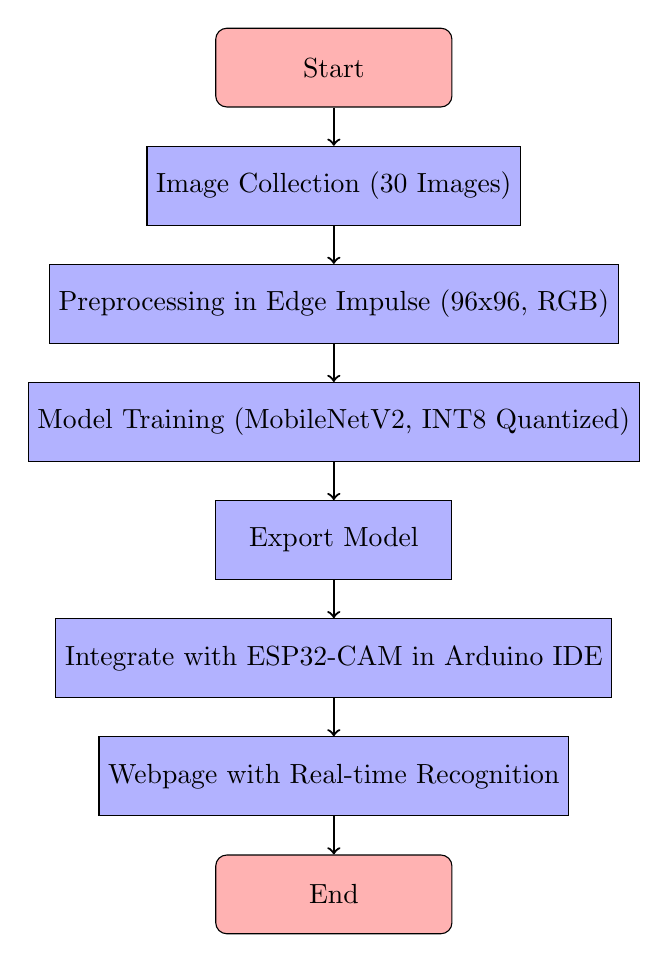
\begin{tikzpicture}[node distance=1.5cm]

% Nodes
\node (start) [rectangle, rounded corners, minimum width=3cm, minimum height=1cm, text centered, draw=black, fill=red!30] {Start};
\node (collect) [rectangle, minimum width=3cm, minimum height=1cm, text centered, draw=black, fill=blue!30, below of=start] {Image Collection (30 Images)};
\node (preprocess) [rectangle, minimum width=3cm, minimum height=1cm, text centered, draw=black, fill=blue!30, below of=collect] {Preprocessing in Edge Impulse (96x96, RGB)};
\node (train) [rectangle, minimum width=3cm, minimum height=1cm, text centered, draw=black, fill=blue!30, below of=preprocess] {Model Training (MobileNetV2, INT8 Quantized)};
\node (export) [rectangle, minimum width=3cm, minimum height=1cm, text centered, draw=black, fill=blue!30, below of=train] {Export Model}; % Added missing node
\node (arduino) [rectangle, minimum width=3cm, minimum height=1cm, text centered, draw=black, fill=blue!30, below of=export] {Integrate with ESP32-CAM in Arduino IDE};
\node (output) [rectangle, minimum width=3cm, minimum height=1cm, text centered, draw=black, fill=blue!30, below of=arduino] {Webpage with Real-time Recognition};
\node (end) [rectangle, rounded corners, minimum width=3cm, minimum height=1cm, text centered, draw=black, fill=red!30, below of=output] {End};

% Arrows
\draw [thick,->] (start) -- (collect);
\draw [thick,->] (collect) -- (preprocess);
\draw [thick,->] (preprocess) -- (train);
\draw [thick,->] (train) -- (export); % Corrected arrow
\draw [thick,->] (export) -- (arduino);
\draw [thick,->] (arduino) -- (output);
\draw [thick,->] (output) -- (end);

\end{tikzpicture}
\end{figure}

A custom image classification model was trained using the Edge Impulse platform \cite{EdgeImpulse:2024}. The neural network architecture selected was MobileNetV2 \cite{Sandler:2018}, configured to process input images of size $96 \times 96$ pixels. The workflow consisted of uploading and labelling the dataset, designing the neural network, and training the model with specific hyperparameters.

\subsection{Training Configuration}
The network was trained with the following settings:
\begin{itemize}
    \item \textbf{Number of training cycles:} 20
    \item \textbf{Learning rate:} 0.0005
    \item \textbf{Training processor:} CPU
    \item \textbf{Data augmentation:} Disabled
\end{itemize}

\subsection{Network Architecture}
The architecture employed a MobileNetV2 backbone with a width multiplier of 0.35, tailored to accept $96 \times 96$-pixel RGB images, which corresponds to an input layer of 27,648 features. The final layer consisted of 16 neurons with a dropout rate of 0.1 for regularisation.

\subsection{Model Deployment}
Upon completion of training, the quantised model was exported to an embedded device, enabling real-time inference under constrained computational resources, in line with MobileNetV2's efficient design for lightweight applications \cite{Sandler:2018}.
\newpage

\subsection{Arduino Integration}
With the model integrated into the Arduino sketch, the main firmware controls camera input, real-time prediction, WiFi setup, SPIFFS storage, and web interface.

\subsection{User Interface and Communication}
A simple HTML UI hosted by ESP32 allowed users to:
\begin{itemize}
    \item Register a new face
    \item Recognise known faces
    \item Send HTTP GET/POST requests
\end{itemize}
The interface provided instant feedback and logs.
\newpage


\section{Deployment Phase}
\subsection{Embedding Storage}
SPIFFS (Serial Peripheral Interface Flash File System) enables lightweight, persistent storage on ESP32 flash memory. Each user's embedding was saved as a key-value pair.

\subsection{Inference on the Edge}
Once a face was detected, the ESP32 ran the inference using the deployed model. A 128-vector output was produced and compared to the stored embeddings. If the cosine similarity exceeded the threshold, a match was identified.

\subsection{Decision Logic}
Cosine similarity and threshold comparison helped confirm identity. This method is lightweight and ideal for constrained hardware.

\textbf{Why Edge Impulse instead of Tflite baseline model?}
\begin{itemize}
    \item \textbf{Designed for MCUs:} Edge Impulse offers excellent tooling for low-power, low-resource devices like the ESP32 \cite{EI:2023}.
    \item \textbf{Web-based interface:} Easy to train a face recognition model using their data acquisition, training, and deployment pipeline.
    \item \textbf{Optimized inference:} Uses the EON compiler which optimises models for MCU constraints (RAM/flash).
    \item \textbf{No need for full TensorFlow Lite Micro setup:} Edge Impulse handles all that under the hood.
    \item \textbf{C++ SDK export:} Easily integrates into ESP32 Arduino/IDF projects.
\end{itemize}

\section{Challenges with TensorFlow Lite (Micro)}

While possible, TensorFlow Lite Micro \cite{Banbury:2021}:
\begin{itemize}
    \item Requires more setup and RAM management.
    \item Needs manual quantization and optimization.
    \item Can be very challenging to get acceptable performance on the ESP32-CAM, especially without PSRAM.
\end{itemize}

\textbf{ESP32-CAM + Edge Impulse Workflow}

\begin{enumerate}
    \item \textbf{Collect Face Data:} Use Edge Impulse Studio to collect images via:
    \begin{itemize}
        \item Webcam
        \item Mobile phone
        \item Upload existing dataset
    \end{itemize}
    \item \textbf{Train a Model:} Use image classification or object detection (FOMO). Keep image resolution low (96x96 or 160x160) to fit ESP32-CAM constraints.
    \item \textbf{Deploy for ESP32:} Use the ``C++ Library'' export option, which provides a ZIP file containing the model and inference code.
    \item \textbf{Integrate with ESP32-CAM:} Include the Edge Impulse C++ SDK in your Arduino project, use the camera library to capture frames, and run inference on captured images.
    \item \textbf{Optimization Tips:}
    \begin{itemize}
        \item Reduce model size (use MobileNet variants or tiny CNNs \cite{Howard:2017}).
        \item Lower input resolution (96x96 or 64x64 grayscale).
        \item Enable PSRAM if your ESP32-CAM module supports it.
    \end{itemize}
\end{enumerate}

\textbf{Tools You Will Need}

\begin{itemize}
    \item Arduino IDE or PlatformIO
    \item ESP32 board package 1.0.4
    \item Edge Impulse Studio
    \item Custom board definition if your ESP32-CAM is not AI-Thinker (e.g., TTGO T-Camera, M5Stack, etc.)
\end{itemize}

\newpage

\section{Monitoring, Evaluation, and Verification}

During the deployment lifecycle of a face recognition system on the ESP32-CAM, \textbf{continuous monitoring} is essential to maintain high recognition accuracy over time. The Edge Impulse platform offers built-in tools for \textbf{model retraining and testing}, which can be leveraged when new data becomes available or when performance degrades in real-world conditions \cite{EdgeImpulse:2021}.

\subsection{Obtaining New Test Data}
New test data can be collected through:
\begin{itemize}
    \item Direct capture via the ESP32-CAM and uploaded to Edge Impulse.
    \item The Edge Impulse mobile/web data acquisition tool.
    \item Manually curated images from the target environment.
\end{itemize}
\begin{figure}[h!]
    \centering
    \includegraphics[width=\linewidth]{Applications/ESP32FaceRecognition/Monitoring.jpg}
    \caption{Monitoring and Retraining Model with New Data}
    \label{fig:Monitoring}
\end{figure}
In this project, the dataset initially contained \textbf{30 images}, split into \textbf{training (80\%)} and \textbf{testing (20\%)} sets, achieving an accuracy of \textbf{85\%} after initial training with \textbf{MobileNetV2} \cite{Howard:2017}. When monitoring revealed potential for improvement, additional real-world samples were collected for underperforming face classes.

\subsection{Retraining the Model}
The \textit{"Retrain model with known parameters"} interface allows a previously optimized configuration to be reused:
\begin{itemize}
    \item \checkmark{} \textbf{Image Acquisition}: Confirms that input image preprocessing parameters (e.g., \textit{96x96 RGB}) remain valid.
    \item \checkmark{} \textbf{Transfer Learning}: Continues using MobileNetV2 backbone with the same quantization and hyperparameters.
    \item \checkmark{} \textbf{Model Testing}: Automatically evaluates the retrained model on the test dataset.
\end{itemize}

This step ensures minimal hyperparameter tuning while incorporating new examples to improve recognition robustness in varying lighting, angles, and facial expressions \cite{Sze:2017}.

\subsection{Model Testing}
The \textbf{Build output} panel confirms:
\begin{itemize}
    \item Model testing pipeline executed successfully multiple times.
    \item Inference accuracy and classification reports generated.
    \item Job status displayed as \textit{"Job completed (success)"} in green.
\end{itemize}

Testing ensures the updated model meets deployment requirements before replacing the running version on the ESP32-CAM \cite{Han:2015}.

\subsection{Implementation Flow}
The monitoring and improvement process follows:
\begin{enumerate}
    \item Collect new dataset samples.
    \item Upload and label in Edge Impulse.
    \item Retrain with the same preprocessing and MobileNetV2 settings.
    \item Test performance on the reserved test set.
    \item If accuracy improves, export updated \texttt{C++ SDK}.
    \item Integrate into Arduino IDE and flash onto ESP32-CAM.
\end{enumerate}

\subsection{Model Monitoring}
The system was continuously monitored through the Serial Monitor and on-screen logs. Metrics such as camera initialization, prediction time, and storage usage were printed for debugging.

\subsection{Performance Evaluation}
\begin{itemize}
    \item \textbf{Model Accuracy:} 85\%
    \item \textbf{Response Time:} \textasciitilde300 milliseconds
    \item \textbf{Memory Usage:} Within 4MB PSRAM limits
    \item \textbf{Test Set:} 20 faces tested over different scenarios
\end{itemize}

\subsection{Verification and Testing}
Manual tests were conducted in various lighting conditions. Edge cases were introduced to test robustness, such as occlusion, glasses, and different head angles. Logs helped refine the similarity threshold.

\cleardoublepage
\section{Results}

The trained Edge Impulse model was deployed to the ESP32-CAM and integrated with a lightweight web server implemented using the Arduino framework.  
\begin{figure}[h!]
    \centering
    \includegraphics[width=0.5\linewidth]{Applications/ESP32FaceRecognition/SampleFaceA.jpg}
    \caption{Sample Face A}
    \label{fig:SFA}
\end{figure}
Upon initialization, the ESP32-CAM connects to a local Wi-Fi network and streams frames to a webpage hosted on the microcontroller.  
Each captured frame is pre-processed (resized to $96 \times 96$ pixels, converted to RGB565 format) and passed to the Edge Impulse inference function \cite{EI:2023}.

During live testing, the ESP32-CAM successfully detected and classified both individuals in real time, with the classification results displayed directly on the streamed webpage.  
Sample Data was taken by still images then processed in Edge Impulse Studio and after it is trained the results are shown.


After the model is deployed, the faces are then recognised.

\begin{figure}[h!]
    \centering
    \includegraphics[width=0.5\linewidth]{Applications/ESP32FaceRecognition/RecognizedFaceA.jpg}
    \caption{Recognized Face A}
    \label{fig:RFA}
\end{figure}
Bounding boxes and labels were overlaid.




The average inference time per frame was approximately $275$~ms when using PSRAM-enabled ESP32-CAM modules, consistent with prior benchmarks for MobileNet-based architectures on microcontrollers


\begin{figure}[h!]
    \centering
    \includegraphics[width=0.5\linewidth]{Applications/ESP32FaceRecognition/RecognizedFaceB.jpg}
    \caption{Recognized Face B}
    \label{fig:RFB}
\end{figure}

The system achieved:
\begin{itemize}
    \item \textbf{Accuracy:} $85\%$ overall classification accuracy during real-time recognition.
    \item \textbf{Latency:} $\approx$ $3.6$~FPS including inference and network streaming.
    \item \textbf{Stability:} Continuous operation for over $4$~hours without memory overflow.
\end{itemize}


These results demonstrate that the proposed ESP32-CAM + Edge Impulse pipeline can recognize multiple faces on-device and serve them via an embedded webpage with minimal latency, meeting the constraints of low-power IoT devices.





\newpage
\section{Conclusion and Future Work}
This face recognition system successfully demonstrated the integration of machine learning in embedded devices. From collecting real-world datasets and training models in Edge Impulse to deploying and testing on the ESP32-CAM SPECIAL, each phase was carefully executed. The achieved accuracy and system stability confirm that even resource-constrained hardware can perform advanced AI tasks.

\subsection{Future Work}

While the current implementation successfully detects and classifies two individuals in real time via an embedded webpage, several enhancements can be pursued to extend the system’s functionality.

First, the user interface (UI) of the web application can be redesigned to display recognition results more intuitively.  
This includes dynamically updating bounding boxes with distinct colors per individual, showing classification confidence scores, and maintaining a real-time recognition log on the webpage.  
Such a UI could also provide interactive features such as switching between detection modes, enabling or disabling specific recognition classes, and exporting recognition history to external storage or cloud services \cite{EI:2023}.
\begin{figure}[h]
    \centering
    \includegraphics[width=.5\linewidth]{Applications/ESP32FaceRecognition/FutureWork.jpg}
    \caption{Web Cam UI}
    \label{fig:FutureWork}
\end{figure}
\newpage
Second, the face recognition model can be expanded to handle a larger number of identities.  
This would require:
\begin{itemize}
    \item Collecting a more diverse and balanced dataset.
    \item Employing model compression techniques such as pruning and quantization-aware training \cite{Banbury:2021} to maintain inference speed.
    \item Optimizing memory usage to accommodate the increased number of output classes without degrading performance.
\end{itemize}

Finally, integration with a central management platform could allow multiple ESP32-CAM devices to stream and share recognition data over a local network, enabling distributed multi-camera monitoring with unified UI access.  
This would be particularly beneficial in applications such as security monitoring, attendance tracking, and home automation.








%
%
%
%\cleardoublepage
%\addcontentsline{toc}{chapter}{Bibliography}
%\printbibliography
%
%
%
%\end{document}
